%%%%%%%%%%%%%%%%%%%%%%%%%%%%%%%%%%%%%%%%%%%%%%%%%%%%%%%
%                File: OpEx_style.tex                 %
%             Created: 2 September 2009               %
%                Updated: 15 May 2015                 %
%                                                     %
%           LaTeX template file for use with          %
%           OSA's journals Optics Express,            %
%             Biomedical Optics Express,              %
%            and Optical Materials Express            %
%                                                     %
%  send comments to Theresa Miller, tmiller@osa.org   %
%                                                     %
% This file requires style file, opex3.sty, under     %
%              the LaTeX article class                %
%                                                     %
%   \documentclass[10pt,letterpaper]{article}         %
%   \usepackage{opex3}                                %
%                                                     %
%                                                     %
%       (c) 2015 Optical Society of America           %
%%%%%%%%%%%%%%%%%%%%%%%%%%%%%%%%%%%%%%%%%%%%%%%%%%%%%%%

%%%%%%%%%%%%%%%%%%%%%%% preamble %%%%%%%%%%%%%%%%%%%%%%%%%%%
\documentclass[10pt,letterpaper]{article}
\usepackage{opex3}
\usepackage{color}
\usepackage{amsmath}
\usepackage{graphicx, subfigure}
\usepackage{threeparttable}
\usepackage{amsfonts}

%%%%%%%%%%%%%%%%%%%%%%% begin %%%%%%%%%%%%%%%%%%%%%%%%%%%%%%
\begin{document}

\title{Quantitative Phase Errors (working title)}

\author{Author A$^{1,*}$, Author B$^{2}$}

\address{$^1$Division of Aerospace Engineering, California Institute of Technology, 1200 E. California Blvd., Pasadena CA 91125, USA\\
$^2$Jet Propulsion Laboratory, California Institute of Technology, 4800 Oak Grove Dr., Pasadena, CA. 91109, USA}

\email{$^*$mbedross@caltech.edu} %% email address is required

% \homepage{http:...} %% author's URL, if desired

%%%%%%%%%%%%%%%%%%% abstract and OCIS codes %%%%%%%%%%%%%%%%
%% [use \begin{abstract*}...\end{abstract*} if exempt from copyright]

\begin{abstract}
This is a placeholder for the abstract. This section will be written as the contents and order of the paper are solidified.
\end{abstract}

\ocis{(000.0000) General.} % REPLACE WITH CORRECT OCIS CODES FOR YOUR ARTICLE, MINIMUM OF TWO; Avoid using the OCIS codes for “General” or “General science” whenever possible.
%For a complete list of OCIS codes, visit: http://www.opticsinfobase.org/submit/ocis/

%%%%%%%%%%%%%%%%%%%%%%% References %%%%%%%%%%%%%%%%%%%%%%%%%F***

\bibliographystyle{plain}
\bibliography{ref}

%%%%%%%%%%%%%%%%%%%%%%%%%%  body  %%%%%%%%%%%%%%%%%%%%%%%%%%
\section{Introduction}

%% Reorganize citations so they appear in numerical order

Quantitative phase imaging is becoming an increasingly common tool used in many academic and research disciplines including astronomy as well as biological microscopy. The use of interferometry for the measurement of angular sizes and separation of astronomical objects was suggested by Armand Hippolyte Louis Fizeau in 1868, but due to challenges related to its practical implementation, it did not become a widely used method until the 1950's to 1970's\cite{tango1980iv}. Phase contrast microscopy was developed in the 1930’s, and remains an important technique in light microscopy\cite{burch1942phase, zernike1934diffraction}. However, phase contrast does not provide quantitative information about the phase shift produced by the object. Methods of quantifying this shift are referred to as quantitative phase imaging (QPI) or quantitative phase microscopy, and are implemented using a variety of interferometric techniques\cite{gureyev1997rapid, lue2007quantitative, cuche1999digital}.\par

Interferometry exploits the wave nature of light in order to create interference between two monochromatic beams. An object in the optical path of one of these beams will distort the wavefront, which results in a a change to the original interference pattern. This change in the interference pattern, or fringe, is used to calculate the phase shift introduced in the light by the object\cite{creath1988v}.Within the previous decade, off-axis digital holographic microscopy (DHM) has increased in use for biological research due to its 3D imaging capabilities in real time as well as its ability to perform quantitative phase measurements.\cite{cuche1999digital, mann2006quantitative, kim2006interference}.\par

Due to the optical setup required in most interferometric devices including off-axis DHM, the measurement of phase introduced by an object is highly susceptible to errors. These errors are in the form of vibrations that cause misalignments of the two beams, laser speckle, temporal phase noise, errors due to uncorrelated noise between the two arms of the interferometer as well as error introduced by the detector used to record the interference pattern.\par

Both pre and post-processing algorithms exist to minimize these errors. The interferometric setup may be optimized by reducing the recording distance and using a detector with smaller pixel sizes\cite{wang2014point}. Other methods to reduce noise include phase error compensation, spatial light modulation (SLM), and multiple frequency overlapping\cite{wang2015new, pan2011coherent, zhang2011coherent, le2015improving, lai2015resolution}, which improve the \textit{contrast} of phase measurements. Noise reduction is also accomplished by filtering certain frequencies, both in the spatial and Fourier planes, with Butterworth filters and masks, respectively\cite{matrecano2015improving, sharma2008improvement, cuche2000spatial}. In addition, efficient encoding methods and correlation based de-noising algorithms have been developed to significantly reduce speckle noise\cite{memmolo2014encoding, molaei2014imaging}. During biological studies, the power of the light source must sometimes be monitored as to not harm the organisms being observed. This has prompted investigation into the reduction of errors introduced by shot noise that becomes significant at low illumination\cite{charriere2006shot, demoli2014digital}. \par

Although the aforementioned de-noising algorithms are effective, a majority of them corrupt the quantitative nature of interferometric phase measurements and result in enhanced phase \textit{contrast} imaging. Due to the, so far, fragmented approach to address and minimize phase errors introduced during interferometric measurements, a unifying error analysis is desirable to analytically investigate the influences of the various sources of error as well as the investigate the manner in which they propagate into the phase calculation of a measurement.\par

 In this work we discuss the theoretical background of interferometry, and common phase calculation algorithms, as well as perform an error analysis on these phase calculation techniques, taking into account various sources of error including photon noise, detector noise, as well as quantization noise. The propagation of these sources of error are investigated in the various phase calculation techniques showing their influence in the resulting phase calculation. These phase error calculations are also applied to the numerical reconstructions of off-axis DHM, which show fundamental similiarities in the method of phase calculations between off-axis DHM and other traditional techniques.

\section{Theory}
Quantitative phase imaging is performed by the use of optical interferometry. This technique encodes both the amplitude characteristics of an object as well as its phase characteristics. It does this with the help of a reference light beam that encodes the unaltered phase of the light before interacting with the object of interest. The reference beam and object beam are recombined at the detector plane which then creates interference patterns, or an interferogram.The beams of an interferometer can be represented as plane waves of identical wavelengths, such that their displacement functions are:

\begin{subequations}
\begin{equation}
 \psi_1(x,y,t)=A_1(x,y)e^{i(\phi_1(x,y)-\omega t)}
 \end{equation}
 \begin{equation}
 \psi_2(x,y,t)=A_2(x,y)e^{i(\phi_2(x,y)-\omega t)}
 \end{equation}
 \end{subequations}
 
 Where $A_1$ and $A_2$ are the amplitudes of the electric field as a function of $x$ and $y$, $\phi_1$ and $\phi_2$ are relative phases of waves 1 and 2 respectively, and $\omega$ is the angular frequency of the wave. 
 
 The combination of these two waves at the detector plane causes the resultant wave to be expressed using the superposition principle such that:
 
 \begin{equation}
 \Psi(x,y,t)=\psi_1+\psi_2=A_1(x,y)e^{i(\phi_1(x,y)-\omega t)}+A_2(x,y)e^{i(\phi_2(x,y)-\omega t)}
 \end{equation}
 
 Modern optical detector arrays' mode of operation is by the integration of the electric field incident on it for a certain period of time. The measured electric field by the detector becomes:
 
 \begin{equation}
 I(x,y)=\int_{t_1}^{t_2}\Psi \Psi^*dt=I_1+I_2+2\sqrt{I_1I_2}\cos(\Delta\phi)
 \label{eq:intensity}
 \end{equation}
 
 Where $\Psi^*$ is the complex conjugate of $\Psi$, $\Delta\phi$ is the phase difference between the two waves, and $I_1$ and $I_2$ are the intensities of beams $1$ and $2$, respectively.\par
 
 With the ability to measure the electric field caused by the superposition of two waves, it is possible to calculate the phase of light at each point of the detector. There are many algorithms that can accomplish this goal and so only three common techniques will be discussed: the Four Bucket/Step Method, the Three Bucket/Step Method, and the Carr\'{e} Method.\par

\subsection{Four Bucket/Step Method}
 
 A common algorithm for the extraction of quantitative phase information from such interferograms, or fringes, is called the `Four Step' or `Four Bucket' Method, where at least four samples must be made per fringe. Figure \ref{fig:fringe} shows a fringe that has been sampled at the four points marked by red triangles. These four points can be sampled at discrete points in space or time, corresponding to a Four Bucket or Four Step method, respectively.\par
 
   In the Four Bucket method, a time invariant interference pattern is sampled across four adjacent pixels that have a phase offset of $\pi/2$ from each other. Similarly, in a Four Step method, an identical pixel experiences a phase step as a function of time such that the light incident on it from exposure $i$ to $i+1$ carries of phase offset of $\pi/2$.
 
 \begin{figure}
 \centering
 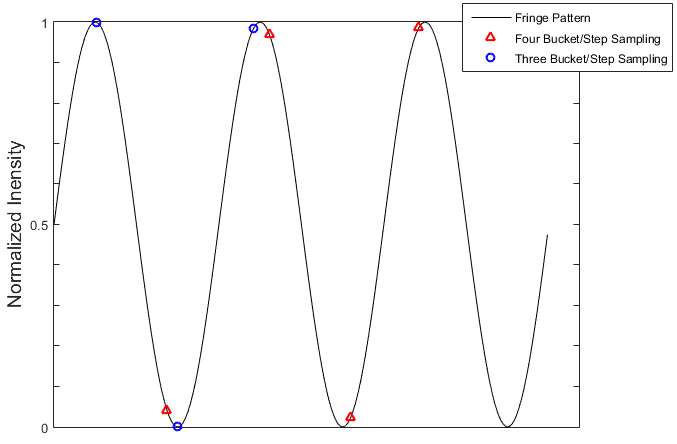
\includegraphics[width=0.8\linewidth]{fringe.png}
 \caption{A fringe that has been sampled at discrete points in space or time according to the four and three bucket/step methods}
 \label{fig:fringe}
 \end{figure}
 
 According to Equation \ref{eq:intensity}, the intensities of the electric field at each of the four sample points are:
 
 \begin{subequations}
\label{eq:fringe}
 \begin{equation}
 I_a=I_1+I_2+2\sqrt{I_1I_2}\cos\phi
 \end{equation}
 \begin{equation}
 I_b=I_1+I_2+2\sqrt{I_1I_2}\cos(\phi+\pi/2)=I_1+I_2-2\sqrt{I_1I_2}\sin\phi
 \end{equation}
 \begin{equation}
 I_c=I_1+I_2+2\sqrt{I_1I_2}\cos(\phi+\pi)=I_1+I_2-2\sqrt{I_1I_2}\cos\phi
 \end{equation}
 \begin{equation}
 I_d=I_1+I_2+2\sqrt{I_1I_2}\cos(\phi+3\pi/2)=I_1+I_2+2\sqrt{I_1I_2}\sin\phi
 \end{equation}
 \end{subequations}
 
 With these equations describing the electric fields of the incident light, the phase difference between the two beams of light ($\phi$) becomes:
 
 \begin{equation}
\label{eq:phase}
\phi=\arctan\left(\frac{\sin\phi}{\cos\phi}\right)=\arctan\left(\frac{I_d-I_b}{I_a-I_c}\right) 
\end{equation}

\subsection{Three Bucket/Step Method}

The Three Bucket/Step Method requires three data points (exposures) in order to calculate the phase of the wavefront. This is accomplished by sampling the fringe pattern at three predefined phase offsets. A common phase offset used is $\pi/2$ from each subsequent exposure. Other phase offsets may be used, such as $\pi/3$, but will not be discussed in detail in this work. \cite{creath1988v} Figure \ref{fig:fringe} shows a fringe that has been sampled at three discrete points in space or time, marked by blue circles. The intensities at each exposure can then be expressed as:

 \begin{subequations}
 \label{eq:3fringe}
 \begin{equation}
 I_a=I_1+I_2+2\sqrt{I_1I_2}\cos\phi
\end{equation}
\begin{equation}
I_b=I_1+I_2+2\sqrt{I_1I_2}\cos(\phi+\pi/2)=I_1+I_2-2\sqrt{I_1I_2}\sin\phi
\end{equation}
\begin{equation}
I_c=I_1+I_2+2\sqrt{I_1I_2}\cos(\phi+\pi)=I_1+I_2-2\sqrt{I_1I_2}\cos\phi
\end{equation}
\end{subequations}

With these equations describing the electric field of an interference pattern, the phase difference can be calculated as:

 \begin{equation}
\label{eq:3phase}
\phi=\arctan\left(\frac{\sin\phi}{\cos\phi}\right)=\arctan\left(\frac{I_c-I_b}{I_a-I_b}\right) 
\end{equation}

\subsection{Carr\'{e} Method}


  Unlike the four or three bucket/step methods that use a fixed and predefined phase offset between exposures, the Carr\'{e} Method allows for phase calculations where the phase offset between exposures can vary linearly. This requires four exposures, each with a phase offset of $\alpha$ between each exposure, where $\alpha\in(0,\pi]$. The four resulting intensities can be expressed as:
  
   \begin{subequations}
\label{eq:Cfringe}
 \begin{equation}
 I_a=I_1+I_2+2\sqrt{I_1I_2}\cos(\phi-3\alpha/2)
 \end{equation}
 \begin{equation}
 I_b=I_1+I_2+2\sqrt{I_1I_2}\cos(\phi-\alpha/2)
 \end{equation}
 \begin{equation}
 I_c=I_1+I_2+2\sqrt{I_1I_2}\cos(\phi+\alpha/2)
 \end{equation}
 \begin{equation}
 I_d=I_1+I_2+2\sqrt{I_1I_2}\cos(\phi+3\alpha/2)
 \end{equation}
 \end{subequations}

The unknown phase shift between exposures ($\alpha$) is calculated using the following expression:

\begin{equation}
\alpha = 2\arctan\left(\sqrt{\frac{3(I_b-I_c)-(I_a-I_d)}{(I_b+I_c)-(I_a+I_d)}}\right)
\end{equation}

With the phase shift between exposures known, the phase of the incident light may be expressed as:

\begin{equation}
\phi = \arctan\left(\frac{\sqrt{3(I_b-I_c)(I_a-I_d)}}{(I_b+I_c)-(I_a+I_d)}\right)
\end{equation}

\subsection{Off-Axis Holography}

A method for the quantitative phase imaging of microscopic matter is the implementation of off-axis digital holographic microscopy (DHM). This technique uses the principles of holography, first developed by Dennis Gabor\cite{Gabor}, to encode the three dimensional morphology of an object onto a single detector plane. Gabor's work related to the recording of holograms onto photosensitive film, but holograms may also be recorded on digital detectors, such as CCD's and CMOS sensors.\par

The morphology of the sample is encoded at the detector plane with the use a `specimen' and `reference' beam of monochromatic light, which is used to create interference patterns. The intensity and phase shift of the light caused by the sample is recorded in these interference patterns.\par

A process of numerical reconstruction is used to propagate the electric field recorded in the digital hologram to a desired focal plane. This allows the real time 3D imaging of dynamic samples in both intensity and phase. A common numerical reconstruction algorithm, called the angular spectrum method, uses the convolution theorem to convolve the hologram with the optical free space propagation term. The complex wavefront ($\Gamma$) as a result of this convolution is thus:

 \begin{equation}
 \Gamma(\xi,\eta)=\mathfrak{F}^{-1}[\mathfrak{F}(h\cdot R)*G]
 \label{eq:recon}
 \end{equation}
 
 Where $h$ is the hologram, $G$ is the free space propagation term, and $\mathfrak{F}$ is the Fourier Transform operator. $R$ is a `phase adjustment' term that is used to remove tilt and other unwanted artifacts from the phase reconstructions. For this rest of this work, the phase adjustment term will be assumed to be unity as phase adjustments can also be made after the reconstruction process.\par
 
   The value and form of the propagation term $G$ depends on the optical setup of the DHM instrument but is always a complex function with a magnitude of unity. The nature of the free space propagation term dictates that it be a pure phaser, which adds diffraction information to the recorded electric field of the hologram. A propagation term used in digital holography is shown in Equation \ref{eq:propa}. It treats optical path length differences in the $x$ and $y$ directions as discrete values due to the finite pixel size of digital detectors.
 
 \begin{equation}
 G(m,n)=\exp\left[\frac{-2\pi di}{\lambda}\sqrt{1-\frac{\lambda^2\left(n+\frac{N_x^2\Delta x^2}{2d\lambda}\right)}{N_x^2\Delta x^2} - \frac{\lambda^2\left(m+\frac{N_y^2\Delta y^2}{2d\lambda}\right)}{N_y^2\Delta y^2}  }\right]
 \label{eq:propa}
 \end{equation}
 
 Where $d$ is the desired focus distance to be reconstructed, $\lambda$ is the wavelength of the illuminating light source, $N_x$ and $N_y$ are the number of pixel on the detector in the $x$ and $y$ directions, and $\Delta x$ and $\Delta y$ are the pixel sizes in the $x$ and $y$ directions, respectively.
 
 The magnitude of $\Gamma(\xi,\eta)$ is the intensity of the incident light at the desired focus distance and the quantitative phase at the desired focus distance is:
 
 \begin{equation}
 \phi=\arctan\left(\frac{\mathfrak{Im}(\Gamma)}{\mathfrak{Re}(\Gamma)}\right)
 \end{equation}
 
 Where $\mathfrak{Im}(\Gamma)$ and $\mathfrak{Re}(\Gamma)$ are the imaginary and real components of $\Gamma$, respectively.\par
 
   It can be seen that the phase calculations of holography are very similar to other interferometric approaches, with the exception that holography involves the convolution of the fringe pattern with a diffraction term to infer on the electric field at different focal plane than the detector.



%\subsection{Phase Unwrapping}

%Due to angles' cyclic nature, phase values obtained from interferometric techniques are bounded between $[0,\pi]$ or $[0,2\pi]$. This gives rise to discontinuities in phase calculations from interferometric techniques. Phase unwrapping algorithms are intended to eliminate the discontinuities in phase signals due to these discontinuities. \par

%Many phase unwrapping algorithms exists and can be categorized as (1) global, (2) regional, and (3) path following algorithms\cite{Herraez:02}. Each type of unwrapping algorithm adds or subtracts the appropriate multiple of the phase range in order to eliminate discontinuities, but each algorithm does this in different ways in order to address different concerns such as image noise, and speckle, as well as to prevent the propagation of phase error.\par

%Common phase unwrapping algorithms include the discrete cosine transform (DCT)\cite{ghiglia:94}, path following\cite{Herraez:02}, and  predetermined conjugate gradient (PCG) techniques\cite{kaufmann:98}.\par

%Each algorithm has its advantages and disadvantages including robustness, computational overhead, and error sensitivity, but because these methods take great care to only add or subtract multiples of the phase bounds and the fact that phase unwrapping is not always necessary, phase unwrapping will be assumed to add negligible error to phase calculations.

\section{QPI Instrumentation}

 Interference patterns can be established by one of many techniques. The fundamental concept behind fringe creation is a difference in path length between two beams of light. This difference in path length can be caused by requiring one beam of light to physically travel further than the other, or by delaying one beam by having it pass through an object with a different index of refraction than the other beam.
 
 There are many experimental setups that can create these necessary interference patterns with which amplitude and phase information can be analyzed. These setups include, but are not limited to, the Michelson, Mach-Zehnder, and the Fabry-P\'{e}rot interferometers. Figure \ref{fig:types} shows optical schematics of each of these interferometers.
 
 \begin{figure}
 \centering
 \subfigure[Michelson Interferometer]{\includegraphics[width=0.45\textwidth]{Michellson1.png}}
 \subfigure[Mach-Zehnder Interferometer]{\includegraphics[width=0.45\textwidth]{Mach-Zehnder1.png}}
 \subfigure[Fabry-P\'{e}rot interferometer]{\includegraphics[width=0.6\textwidth]{Fabry-Perot1.png}}
 \label{fig:types}
 \caption{Optical schematics of various interferometer types}
 \end{figure}
 
 %\subsection{Holography}
 
%The application of holography to interferometric techniques results in off-axis holography. 
 
% In-line holography is a single beam holographic setup. A single coherent light source is used to illuminate a sample of interest. The coherent light interacts with the sample by being absorbed and/or diffracted. The light interactions are recorded at a detector plane, which captures the samples three-dimensional morphology. Because this method does not use a reference beam, quantitative phase is not possible with this method, although it was reported by P. Spanne, et al.\cite{spanne1999line} that phase \textit{contrast} microscopy is possible by obtaining out of focus in-line holographic images.

 
\section{Phase Errors and Noise}

As with any measurement, there are errors and noise that must be accounted for. In the application of quantitative phase imaging, digital sensors that measure the intensity of incident light are subject to multiple sources of error. These sources of error include photon noise, dark noise, read noise, quantization noise, pixel non-uniformity, as well as electronic interference. Such errors as pixel non-uniformity, and electronic interference are difficult to quantify due to their dependence on factors that are independent to the optical system. As a result, they will only be mentioned here.\par

Photon noise is a fundamental trait of light and is caused by the discrete nature of photons. This noise is modeled as a Poisson process where the noise is equal to the square root of the number of photons incident on the pixel ($\sqrt{I}$).

Dark noise is the false reading of photons by the sensor due to thermally generated electrons on the sensor array. Dark noise is typically specified by the manufacturer of the sensor array and camera and is reported in units of electrons (RMS) per pixel per second of integration.\par

Read noise is the combinations of all `on chip' sources of error. In many cameras, on chip processes occur prior to the image data being sent to a computer, the errors introduced as a result of this processing are quantified and combined by sensor and camera manufacturers and reported in units of electrons (RMS) per read.\par

Quantization noise arises from any analog to digital conversion. In the case of an optical detector, photons are used to generate electrons in each pixel. These electrons build up voltage, which is then counted and converted to a digital number to be stored by the computer. The error of a digitization process has a mean of zero and extrema of $\pm0.5L_{SB}$, where $L_{SB}$ is the least significant bit of the analog to digital converter (ADC). The standard deviation of this error is $L_{SB}/\sqrt{12}$ and is commonly used to quanitfy errors introduced as a result of digitization of an analog signal.

The manufacture of sensor arrays are highly controlled and repeatable processes but there is inevitably irregularity in the manufacturing process. Pixel non-uniformity is the error introduced as a result of non-uniform sensitivity to light from one pixel to another on a detector array.\par

Other errors can be introduced into the measurement of light in the form of electronic interference from nearby uninsulated devices. If a strong enough electronic interference is present prior to the signal amplifiers of the sensor, the interference noise will be proportionally amplified and corrupt the signal being measured.\par

For the following analyses, the error in the measurement of the light intensity incident on a particular pixel will be the root sum square (RSS) off all the contributing noise sources, and will be considered equal between all pixels. Thus, the error of an electric field intensity measurement is:

\begin{equation}
\label{eq:intense}
\delta I_i=\sqrt{I_i+(\Delta t\delta D)^2+M(\delta R)^2+\frac{L_{SB}^2}{12}}
\end{equation}

Where $I_i$ is the number of photons incident on pixel $i$, $\Delta t$ is the integration time of the pixel, $\delta D$ is the dark noise, $\delta R$ is the read noise, and $M$ is the number of reads taken to make the measurement.

\subsection{Four Bucket/Step Method}

	Beginning with the equations for the electric field intensities at four points along a fringe in Equation \ref{eq:fringe}, and its resulting equation for phase in Equation \ref{eq:phase}, we apply the equation for the propagation of error. The equation for phase variance is thus:

\begin{equation}
\label{eq:propo}
\delta\phi^2=\sum_{i=1}^4\left(\frac{\partial \phi}{\partial I_i}\right)^2\delta I_i^2
\end{equation}

The partial differentials of phase with respect to each intensity function are:

\begin{subequations}
\begin{equation}
\label{eq:diffA4}
\frac{\partial \phi}{\partial I_a}=-\frac{\partial \phi}{\partial I_c}=\frac{I_b-I_d}{(I_a-I_c)^2+(I_d-I_b)^2}
\end{equation}
\begin{equation}
\label{eq:diffB4}
\frac{\partial \phi}{\partial I_b}=-\frac{\partial \phi}{\partial I_d}=\frac{I_c-I_a}{(I_a-I_c)^2+(I_d-I_b)^2}
\end{equation}
\end{subequations}

Combining Equations \ref{eq:propo}, \ref{eq:diffA4}, and \ref{eq:diffB4}, with the expression for intensity errors of Equation \ref{eq:intense} yields:

\begin{equation}
\delta_\phi^2=\frac{I_1+I_2+2\left((\Delta t\delta D)^2+M(\delta R)^2+\frac{L_{SB}^2}{12}\right)}{4I_1I_2}
\end{equation}

Fringe visibility is measure of contrast in the recorded interference pattern by the detector array. Fringe visibility is defined as the amplitude of the fringe divided by the mean fringe value.

\begin{equation}
\label{eq:vis}
V=\frac{2\sqrt{I_1I_2}}{I_1+I_2}
\end{equation}

With Equation \ref{eq:vis}, the expression for phase noise becomes:

\begin{equation}
\label{eq:phaseNoise}
\delta_\phi=\sqrt{\frac{1}{2V^2<I>}+\frac{2\left((\Delta t\delta D)^2+M(\delta R)^2+\frac{L_{SB}^2}{12}\right)}{2V^2(<I>)^2}}
\end{equation}

Where $<I>$ is the average electric field intensity across the fringe.\par

Equation \ref{eq:phaseNoise}, provides an expression for the error propagated by the four step method  as a result of photon, detector, and quantization noise. Note that the above expression consists of two terms on the right hand side of Equation \ref{eq:phaseNoise}. The left most corresponds to errors as a result of photon noise, which will be present in any optical system due to the discrete nature of light, and the right corresponds to errors that are propagated into the phase measurement as a result of the detector used to make intensity measurements.\par

\subsection{Three Bucket/Step Method}

For the Three Bucket/Step Method, the propagation of error equation is written as:

\begin{equation}
\label{eq:3propo}
\delta\phi^2=\sum_{i=1}^3\left(\frac{\partial \phi}{\partial I_i}\right)^2\delta I_i^2
\end{equation}

The partial derivatives of phase with respect to the three intensities (Equation \ref{eq:3fringe}) are:

\begin{subequations}
\label{eq:3deriv}
\begin{equation}
\label{eq:3diffA}
\frac{\partial \phi}{\partial I_a}=\frac{I_b-I_c}{(I_a-I_b)^2+(I_c-I_b)^2}
\end{equation}
\begin{equation}
\label{eq:3diffB}
\frac{\partial \phi}{\partial I_b}=\frac{I_c-I_a}{(I_a-I_b)^2+(I_c-I_b)^2}
\end{equation}
\begin{equation}
\label{eq:3diffC}
\frac{\partial \phi}{\partial I_c}=\frac{I_a-I_b}{(I_a-I_b)^2+(I_c-I_b)^2}
\end{equation}
\end{subequations}

Combining Equations \ref{eq:intense}, \ref{eq:3propo}, \ref{eq:3deriv}, as well as the definition of fringe visibility in Equation \ref{eq:vis}, results in the following expression for phase variance due to the three bucket/step method.

\begin{equation}
\label{eq:3error}
\delta\phi = \sqrt{\frac{1+2\cos^2\phi-2V\sin\phi\cos^2\phi}{4V^2<I>}+\frac{3\left((\Delta t\delta D)^2+M(\delta R)^2+\frac{L_{SB}^2}{12}\right)(1-\sin(2\phi))}{16V^2(<I>)^2}}
\end{equation}

From Equation \ref{eq:3error} it can be seen that the phase error present in the Three Bucket/Step Method is not constant, but is a function of the phase being measured. This is unlike the Four Bucket/Step Method where the phase errors are independent of the magnitude of phase being measured.

\subsection{Carr\'{e} Method}

Implementing the equation for the propagation of error to the Carr\'{e} Method of phase calculation, the phase variance is:

\begin{equation}
\label{eq:Cpropo}
\delta\phi^2=\sum_{i=1}^4\left(\frac{\partial \phi}{\partial I_i}\right)^2\delta I_i^2
\end{equation}

The partial derivatives of phase with respect to the four recorded intensities defined in Equation \ref{eq:Cfringe} are:

\begin{subequations}
\label{eq:Cderiv}
\begin{equation}
\label{eq:diffA}
\frac{\partial \phi}{\partial I_a}=-\frac{\partial \phi}{\partial I_d}=\frac{\left(\frac{3(I_b-I_c)[(I_b+I_c)-(I_a+I_d)]}{2\sqrt{3(I_b-I_c)(I_a-I_d)}}\right)+\sqrt{3(I_b-I_c)(I_a-I_d)}}{\left((I_b+I_c)-(I_a+I_d)\right)^2+3(I_b-I_c)(I_a-I_d)}
\end{equation}
\begin{equation}
\label{eq:diffB}
\frac{\partial \phi}{\partial I_b}=-\frac{\partial \phi}{\partial I_c}=\frac{\left(\frac{3(I_a-I_d)[(I_b+I_c)-(I_a+I_d)]}{2\sqrt{3(I_b-I_c)(I_a-I_d)}}\right)+\sqrt{3(I_b-I_c)(I_a-I_d)}}{\left((I_b+I_c)-(I_a+I_d)\right)^2+3(I_b-I_c)(I_a-I_d)}
\end{equation}
\end{subequations}

Because the partial derivatives of $\phi$ with respect to $I_a$ and $I_d$, as well as $I_b$ and $I_c$ are odd functions of each other, respectively, the variance of phase reduces to:

\begin{equation}
\label{eq:Cpropo}
\delta\phi^2=\left(\frac{\partial \phi}{\partial I_a}\right)^2(\delta I_a^2+\delta I_d^2)+\left(\frac{\partial \phi}{\partial I_b}\right)^2(\delta I_b^2+\delta I_c^2)
\end{equation}

Combining Equations \ref{eq:intense}, \ref{eq:Cderiv} and \ref{eq:Cpropo}, yields the following expression for phase variance of the Carr\'{e} Method for phase calculation using an unknown phase shift.

\begin{multline}
\label{eq:CpropoFull}
\delta\phi^2 =\frac{A\left(\frac{3D(B-A)}{2\sqrt{3CD}}+\sqrt{3CD}\right)+B\left(\frac{3C(B-A)}{2\sqrt{3CD}}+\sqrt{3CD}\right)}{(B-A)^2+3CD}\\
+\frac{2\left((\Delta t\delta D)^2+M(\delta R)^2+\frac{L_{SB}^2}{12}\right)\left[(3D(B-A)+6CD)^2+(3C(B-A)+6CD)^2\right]}{12CD((B-A)+6CD)^2}
\end{multline}

Where,

\begin{subequations}
\begin{equation}
A=I_a+I_d=2(I_1+I_2)+4\sqrt{I_1I_2}\cos\phi\cos\left(\frac{3\alpha}{2}\right)
\end{equation}
\begin{equation}
B=I_b+I_c=2(I_1+I_2)+4\sqrt{I_1I_2}\cos\phi\cos\left(\frac{\alpha}{2}\right)
\end{equation}
\begin{equation}
C=I_a-I_d=4\sqrt{I_1I_2}\sin\phi\sin\left(\frac{3\alpha}{2}\right)
\end{equation}
\begin{equation}
D=I_b-I_c=4\sqrt{I_1I_2}\sin\phi\sin\left(\frac{\alpha}{2}\right)
\end{equation}
\end{subequations}

From Equation \ref{eq:CpropoFull} it is clear that sampling a fringe of an interferogram at unknown but constant intervals adds a great deal of complexity to the error of the calculation. 
%In a trivial case, if $\alpha=\pi$, the error of using this method reduces to:

%\begin{equation}
%\delta_\phi=\frac{I_1+I_2}{12\sqrt{I_1I_2}\sin\phi}=\frac{1}{6V\sin\phi}
%\end{equation}

\subsection{Off-Axis Holography}

To quantify the phase errors present in the numerical reconsrtuction of off-axis holography, attention must be paid to the reconstruction process itself. \par

Due to the discrete nature of recorded holograms, the analytical form of the Fourier Transform cannot be used, in its place, the discrete Fourier Transform (DFT) must be implemented. The discrete Fourier Transform ($F_k$) of a discrete signal ($f_n$) is defined as:

\begin{equation}
F_k=\sum_{n=0}^{N-1}f_n\cdot \exp\left[\frac{-2\pi ikn}{N}\right]
\label{eq:DFT}
\end{equation}

Where $N$ is the length of the signal. Assume that the fringes established at the detector plane, and recorded in the hologram are sampled such that there are four samples per fringe, similar to the four step/bucket method. A sample frequency of three to four samples per period of a cyclic signal is a common sample rate due to the Shannon-Nyquist sampling theorem. In the case where $N=4$. Equation \ref{eq:DFT} can be represented in matrix form.

\begin{equation}
\left[
\begin{matrix}
F_0\\
F_1\\
F_2\\
F_3
\end{matrix}
\right]
=
\left[
\begin{matrix}
1 & 1 & 1 & 1\\
1 & -i & -1 & i\\
1 & -1 & 1 & -1\\
1 & i & -1 & -i
\end{matrix}
\right]
\left[
\begin{matrix}
f_0\\
f_1\\
f_2\\
f_3
\end{matrix}
\right]
\end{equation}

The inverse DFT algorithm is as follows:

\begin{equation}
f_n=\sum_{k=0}^{N-1}F_k\cdot \exp\left[\frac{+2\pi ikn}{N}\right]
\label{eq:iDFT}
\end{equation}

Which, for a signal of length four, can be expressed in matrix form as:

\begin{equation}
\left[
\begin{matrix}
f_0\\
f_1\\
f_2\\
f_3
\end{matrix}
\right]
=
\left[
\begin{matrix}
1 & 1 & 1 & 1\\
1 & i & -1 & -i\\
1 & -1 & 1 & -1\\
1 & -i & -1 & i
\end{matrix}
\right]
\left[
\begin{matrix}
F_0\\
F_1\\
F_2\\
F_3
\end{matrix}
\right]
\end{equation}

For a fringe that has been sampled at four equally spaced points, the values recorded at each of the four pixels is identical to Equation \ref{eq:fringe}. The DFT of the recorded fringe($h_n$) is:

\begin{equation}
\left[
\begin{matrix}
H_0\\
H_1\\
H_2\\
H_3
\end{matrix}
\right]
=
\left[
\begin{matrix}
4(I_1+I_2)\\
2(I_1+I_2)+(4\sqrt{I_1I_2}\sin\phi)i\\
0\\
(4\sqrt{I_1I_2}\cos\phi)-(4\sqrt{I_1I_2}\sin\phi)i
\end{matrix}
\right]
\end{equation}


\end{document}
